\documentclass[9pt, handout]{beamer}
\usetheme{CambridgeUS}
\usepackage{xcolor}
\usepackage{geometry}
\usepackage{array}
\usepackage{comment}

\AtBeginSection[]
{
  \begin{frame}
    \frametitle{Table of Contents}
    \tableofcontents[currentsection]
  \end{frame}
}

\setbeamertemplate{footline}
{
  \leavevmode%
  \hbox{%
    \begin{beamercolorbox}[wd=.333333\paperwidth,ht=2.25ex,dp=1ex,center]{author in head/foot}%
      \usebeamerfont{author in head/foot}\insertshortauthor
    \end{beamercolorbox}%
    \begin{beamercolorbox}[wd=.333333\paperwidth,ht=2.25ex,dp=1ex,center]{title in head/foot}%
      \usebeamerfont{title in head/foot}\insertshortsubtitle
    \end{beamercolorbox}%
    \begin{beamercolorbox}[wd=.333333\paperwidth,ht=2.25ex,dp=1ex,right]{date in head/foot}%
      \usebeamerfont{date in head/foot}\insertshortdate{}\hspace*{2em}
      \usebeamertemplate{page number in head/foot}\hspace*{2ex}
    \end{beamercolorbox}
  }%
  \vskip0pt%
}

\title{Principles of Economics}
\subtitle{Discussion Session 2: Elasticity}
\author{Joe Wilske and Yuzhi Yao}
\institute{Boston College}
\date{\today}

\begin{document}

\frame{\titlepage}

\begin{frame}{Slope vs Elasticity}

    We want to describe the effect of a change in price on quantity.\\

    Two options:
    \begin{enumerate}
        \item Slope:
        \begin{itemize}
            \item Ratio of the \textit{absolute} change in $f(x)$ to the \textit{absolute} change in $x$.
            \item Interpretation: ``If $x$ increases by 1, then $f(x)$ increases by $m$."
            \item \[m = \frac{f(x_2) - f(x_1)}{x_2 - x_1}\]
        \end{itemize}
        \item Elasticity:
        \begin{itemize}
            \item Ratio of the \textit{proportional} change in $f(x)$ to the \textit{proportional} change in $x$.
            \item Interpretation: ``If $x$ increases by 1\%, then $f(x)$ increases by $\varepsilon$\%."
            \item \[\varepsilon = \frac{\Big(\frac{f(x_2) - f(x_1)}{\textcolor{darkred}{midpoint(f(x_1), f(x_2))}}\Big)}{\Big(\frac{x_2 - x_1}{\textcolor{darkred}{midpoint(x_1, x_2)}}\Big)}\]
        \end{itemize}
    \end{enumerate}
\end{frame}

\begin{frame}{So why use elasticity?}

    Elasticity allows us to compare markets where prices/quantities are quite different:
    \begin{figure}
        \centering
        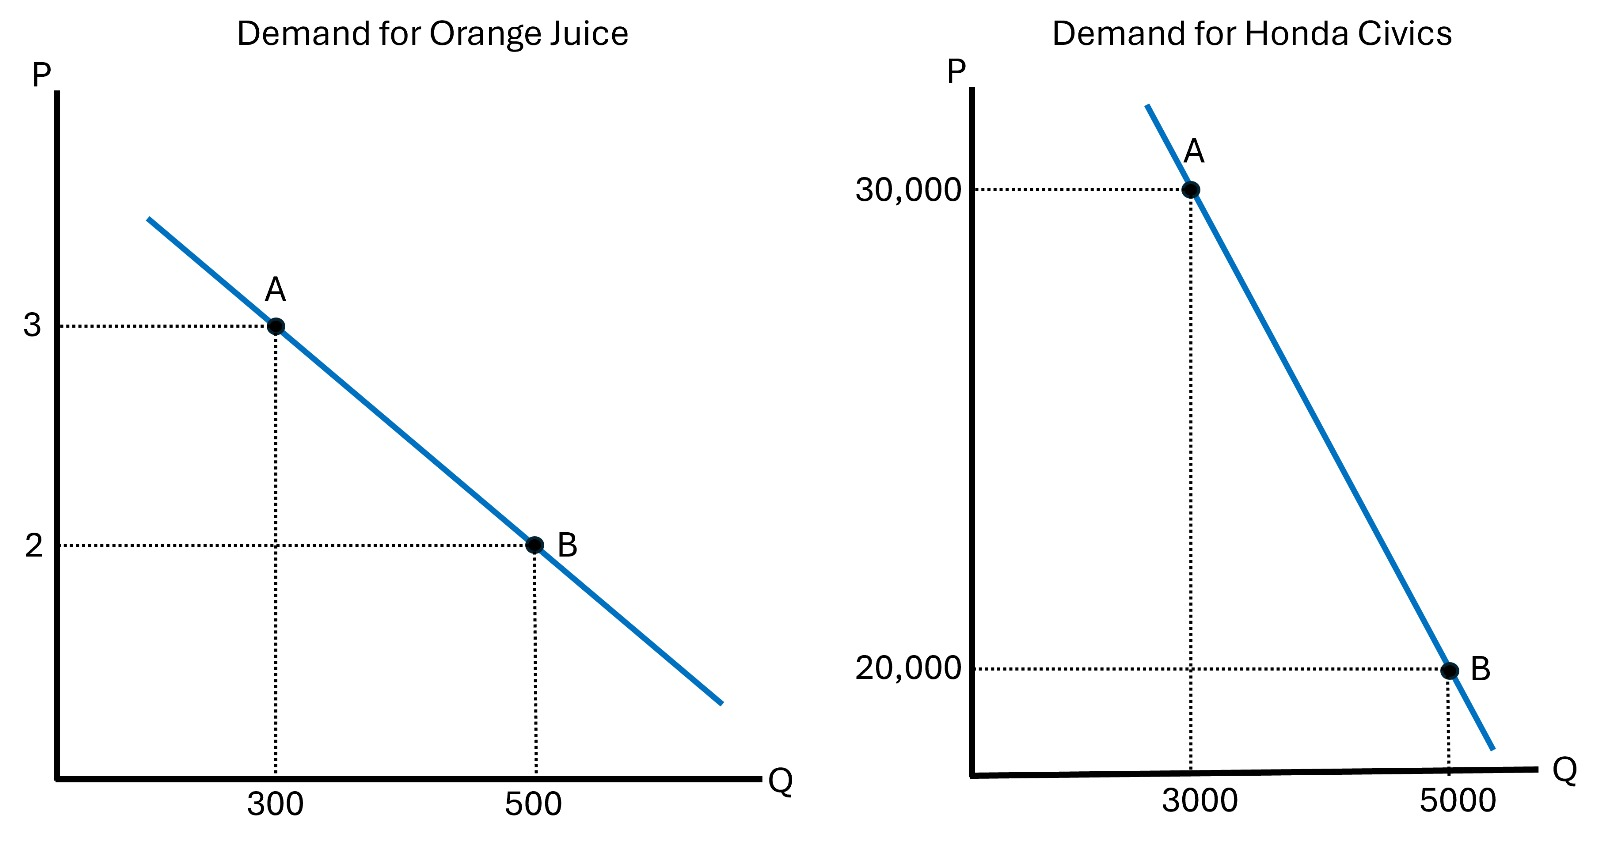
\includegraphics[width=.8\linewidth]{demand_curve_comparison.jpg}
        \label{fig:demand_curve_comparison}
    \end{figure}
    \begin{itemize}
        \item Slopes: $\quad m_{OJ} = -200, \quad m_{HC} = -0.2$
        \item Elasticities: $\quad \varepsilon_{OJ} = 1.25, \quad \varepsilon_{HC} = 1.25$
        \item How do we interpret these numbers? (``If $P$ increases by 1, then...")
    \end{itemize}
\end{frame}

\begin{frame}{More interpretation}
    \begin{itemize}
    \item If demand is elastic ($\varepsilon > 1$), then a change in $P$ causes a proportionately \textbf{large} change in $Q$.
    \vspace{5}
    \item If demand is inelastic ($\varepsilon < 1$), then a change in $P$ causes a proportionately \textbf{small} change in $Q$.
    \vspace{5}
    \item If demand is unit-elastic ($\varepsilon = 1$), then a change in $P$ causes a proportionately \textbf{equal} change in $Q$.
    \end{itemize}
\end{frame}

\begin{frame}{Exercise 1: Price Elasticity of Demand}
    Suppose the current price of coffee sold at Hillside Cafe is \$5 per cup. However, the cafe announced this Friday that the price of coffee per cup will be \$3. The cafe expects that after reducing the price, the number of cups sold will increase from 200 to 400. 
    \begin{enumerate}
        \item Using the midpoint formula, calculate the price elasticity of demand for coffee between \$5 and \$3. Is the demand elastic, inelastic, or unit elastic?
        \item What will happen to the total revenue of Hillside Cafe? Please answer by calculating the change in total revenue and explain why.
        \item In which direction do you expect the total revenue will change if Hillside Cafe cuts the price during the final week? Why?
        \item \textit{Bonus:} What is the elasticity of demand at the revenue-maximizing price?
    \end{enumerate}
    \vspace{1.5in}
\end{frame}

\begin{frame}{Exercise 1: Price Elasticity of Demand}
    Solution: 
    \begin{enumerate}
        \item $\frac{4}{3}$. Elastic.  
        \item Total revenue changes from \$1000 to \$1200. Lowering the price will increase revenue if demand is relatively elastic. 
        \item Total revenue will decrease as the seller lowers the price when the demand is inelastic.
        \item \textit{Bonus:} Revenue is maximized when $\varepsilon = 1$! \\
        If $\varepsilon < 1$, the seller can increase revenue by increasing the price, which increases $\varepsilon$.\\
        If $\varepsilon > 1$, the seller can increase revenue by decreasing the price, which decreases $\varepsilon$.\\
        Thus, revenue is maximized when $\varepsilon = 1$.
    \end{enumerate}
\end{frame}

\begin{frame}{Exercise 2: Price Elasticity of Supply}
    Suppose Anirudh and Jae work at Hillside Cafe with an hourly wage of \$15. Both of them work 4 hours per day. Now the manager wants to extend the operating hours and announces to increase the wage to \$20. Anirudh is willing to work 6 hours with the new wage offered, but Jae only wants to work 5 hours. 
    \begin{enumerate}
        \item Using the midpoint formula, calculate the price elasticity of supply for Anirudh and Jae between \$15 and \$20.  
        \item What should Anirudh's supply curve look like? What about Jae's?  
    \end{enumerate}
    \vspace{1.5in}
\end{frame}

\begin{frame}{Exercise 2: Price Elasticity of Supply}
    Solution: 
    \begin{enumerate}
        \item Anirudh: $\frac{7}{5}$; Jae: $\frac{7}{9}$
        \item Since Anirudh's supply is elastic while Jae's supply is inelastic, Anirudh's supply curve should be flatter than Jae's. 
    \end{enumerate}
\end{frame}


\end{document}

